
\cxset{style53/.style={
 chapter name= CHAPTER,
 numbering=Roman,
% number font-size=Large,
% number font-family=rmfamily,
% number before=,
% number after=,
% number dot=,
 %number position=rightname,
% number float=center,
% number display=block,
 number color=sweet,
 chapter color=black,
 chapter font-size=Large,
 chapter before=,
 chapter after=,
 chapter margin-left=0pt,
 title font-family=rmfamily,
 % set title parameters
 title font-color=spot!50,
 title font-weight=bold,
 title font-face=tiresias,
 title font-family=serif,
 title font-size=huge,
 title font-shape =itshape,
 title before=,
 title padding-right=0pt,
 title padding-left=0pt,
 title border-width=2pt,
 title border-color = orange,
 title border-left-color = blue,
 chapter title text-align = Centering,
 title display=block,
 title float = right,
 chapter title width=0.8\textwidth,
 title beforeskip=,
 title after=,
 header style=empty}}

\cxset{style53}

\chapter{VAULT OF THE AGES STYLE FIFTY THREE}


The book alleges the discovery of Jesus tomp \cite{style53}. True or not, the book eloquently describes  life in Israel in the early years of the second millenium.\footnote{From \textit{The
Jesus
Family
Tomb,   
The Discovery, the Investigation,
and the Evidence
That Could Change History}, 
Simcha Jacobovici and Charles Pellegrino
Harper Collins.}

Simcha Jacobovici and Charles
Pellegrino have carried out and delivered evidence based on their own investigations to 
connect a first-century Jewish tomb found in Talpiot, Jerusalem,
in 1980 to the tomb of Jesus and his family. They also provide physical evidence from within the tomb says about Jesus, his death, and his relationships with the other family members found in
the same burial site. I read the book and remained unconvinced. 

\begin{figure}[ht]
\fbox{%
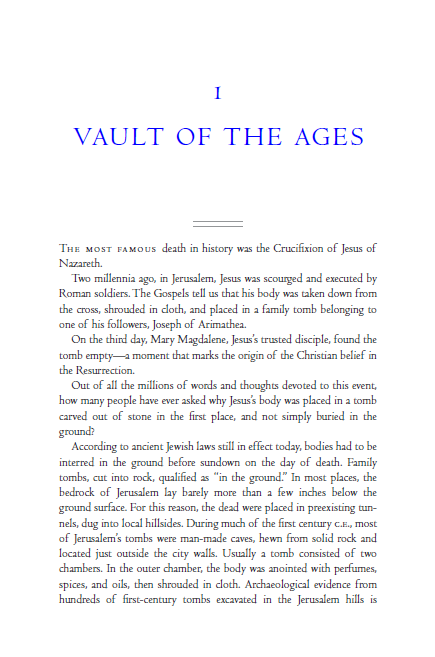
\includegraphics[width=0.48\textwidth]{./chapters/chapter53}\hfill
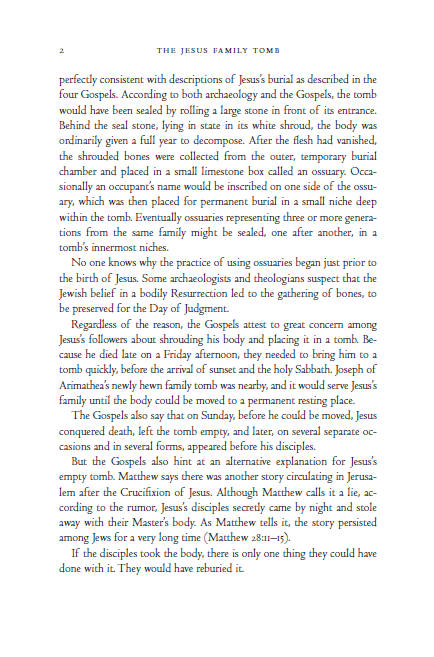
\includegraphics[width=0.48\textwidth]{./chapters/chapter53a}}
\caption{Style 53 Page spread.}
\end{figure}

The book is written for the wide public and although it does provides references 
\lipsum

\section{Illustrations}

Illustrations less than the width of the textblock are set with a sideways caption.

\begin{figure}[ht]
\includegraphics[width=\textwidth]{jesus}
\caption{Style 53 Image pages.}
\end{figure}
\lipsum[1-4]

\cxset{chapter opening = anywhere}

\cxset{chapter float=none,
          title float=none,
          title margin-left=0pt}

\chapter{The Vault of the Ages}

\cxset{chapter float=center,
          title display=block,
          title float=center,
          title margin-top=20pt}

\chapter{The Vault of the Ages}

\cxset{chapter float=none,
         chapter name=none,
          title float=right,
          title display=none,
          title margin-left=28pt}

\chapter{The Vault of the Ages}





